% Template for PLoS
% Version 3.5 March 2018
%
% % % % % % % % % % % % % % % % % % % % % %
%
% -- IMPORTANT NOTE
%
% This template contains comments intended
% to minimize problems and delays during our production
% process. Please follow the template instructions
% whenever possible.
%
% % % % % % % % % % % % % % % % % % % % % % %
%
% Once your paper is accepted for publication,
% PLEASE REMOVE ALL TRACKED CHANGES in this file
% and leave only the final text of your manuscript.
% PLOS recommends the use of latexdiff to track changes during review, as this will help to maintain a clean tex file.
% Visit https://www.ctan.org/pkg/latexdiff?lang=en for info or contact us at latex@plos.org.
%
%
% There are no restrictions on package use within the LaTeX files except that
% no packages listed in the template may be deleted.
%
% Please do not include colors or graphics in the text.
%
% The manuscript LaTeX source should be contained within a single file (do not use \input, \externaldocument, or similar commands).
%
% % % % % % % % % % % % % % % % % % % % % % %
%
% -- FIGURES AND TABLES
%
% Please include tables/figure captions directly after the paragraph where they are first cited in the text.
%
% DO NOT INCLUDE GRAPHICS IN YOUR MANUSCRIPT
% - Figures should be uploaded separately from your manuscript file.
% - Figures generated using LaTeX should be extracted and removed from the PDF before submission.
% - Figures containing multiple panels/subfigures must be combined into one image file before submission.
% For figure citations, please use "Fig" instead of "Figure".
% See http://journals.plos.org/plosone/s/figures for PLOS figure guidelines.
%
% Tables should be cell-based and may not contain:
% - spacing/line breaks within cells to alter layout or alignment
% - do not nest tabular environments (no tabular environments within tabular environments)
% - no graphics or colored text (cell background color/shading OK)
% See http://journals.plos.org/plosone/s/tables for table guidelines.
%
% For tables that exceed the width of the text column, use the adjustwidth environment as illustrated in the example table in text below.
%
% % % % % % % % % % % % % % % % % % % % % % % %
%
% -- EQUATIONS, MATH SYMBOLS, SUBSCRIPTS, AND SUPERSCRIPTS
%
% IMPORTANT
% Below are a few tips to help format your equations and other special characters according to our specifications. For more tips to help reduce the possibility of formatting errors during conversion, please see our LaTeX guidelines at http://journals.plos.org/plosone/s/latex
%
% For inline equations, please be sure to include all portions of an equation in the math environment.
%
% Do not include text that is not math in the math environment.
%
% Please add line breaks to long display equations when possible in order to fit size of the column.
%
% For inline equations, please do not include punctuation (commas, etc) within the math environment unless this is part of the equation.
%
% When adding superscript or subscripts outside of brackets/braces, please group using {}.
%
% Do not use \cal for caligraphic font.  Instead, use \mathcal{}
%
% % % % % % % % % % % % % % % % % % % % % % % %
%
% Please contact latex@plos.org with any questions.
%
% % % % % % % % % % % % % % % % % % % % % % % %

\documentclass[10pt,letterpaper]{article}
\usepackage[top=0.85in,left=2.75in,footskip=0.75in]{geometry}

% amsmath and amssymb packages, useful for mathematical formulas and symbols
\usepackage{amsmath,amssymb}

% Use adjustwidth environment to exceed column width (see example table in text)
\usepackage{changepage}

% Use Unicode characters when possible
\usepackage[utf8x]{inputenc}

% textcomp package and marvosym package for additional characters
\usepackage{textcomp,marvosym}

% cite package, to clean up citations in the main text. Do not remove.
% \usepackage{cite}

% Use nameref to cite supporting information files (see Supporting Information section for more info)
\usepackage{nameref,hyperref}

% line numbers
\usepackage[right]{lineno}

% ligatures disabled
\usepackage{microtype}
\DisableLigatures[f]{encoding = *, family = * }

% color can be used to apply background shading to table cells only
\usepackage[table]{xcolor}

% array package and thick rules for tables
\usepackage{array}

% create "+" rule type for thick vertical lines
\newcolumntype{+}{!{\vrule width 2pt}}

% create \thickcline for thick horizontal lines of variable length
\newlength\savedwidth
\newcommand\thickcline[1]{%
  \noalign{\global\savedwidth\arrayrulewidth\global\arrayrulewidth 2pt}%
  \cline{#1}%
  \noalign{\vskip\arrayrulewidth}%
  \noalign{\global\arrayrulewidth\savedwidth}%
}

% \thickhline command for thick horizontal lines that span the table
\newcommand\thickhline{\noalign{\global\savedwidth\arrayrulewidth\global\arrayrulewidth 2pt}%
\hline
\noalign{\global\arrayrulewidth\savedwidth}}


% Remove comment for double spacing
%\usepackage{setspace}
%\doublespacing

% Text layout
\raggedright
\setlength{\parindent}{0.5cm}
\textwidth 5.25in
\textheight 8.75in

% Bold the 'Figure #' in the caption and separate it from the title/caption with a period
% Captions will be left justified
\usepackage[aboveskip=1pt,labelfont=bf,labelsep=period,justification=raggedright,singlelinecheck=off]{caption}
\renewcommand{\figurename}{Fig}

% Use the PLoS provided BiBTeX style
% \bibliographystyle{plos2015}

% Remove brackets from numbering in List of References
\makeatletter
\renewcommand{\@biblabel}[1]{\quad#1.}
\makeatother



% Header and Footer with logo
\usepackage{lastpage,fancyhdr,graphicx}
\usepackage{epstopdf}
%\pagestyle{myheadings}
\pagestyle{fancy}
\fancyhf{}
%\setlength{\headheight}{27.023pt}
%\lhead{
\includegraphics[width=2.0in]{PLOS-submission.eps}}
\rfoot{\thepage/\pageref{LastPage}}
\renewcommand{\headrulewidth}{0pt}
\renewcommand{\footrule}{\hrule height 2pt \vspace{2mm}}
\fancyheadoffset[L]{2.25in}
\fancyfootoffset[L]{2.25in}
\lfoot{\today}

%% Include all macros below

\newcommand{\lorem}{{\bf LOREM}}
\newcommand{\ipsum}{{\bf IPSUM}}


% Pandoc citation processing

\usepackage{booktabs}
\usepackage{longtable}
\usepackage{array}
\usepackage{multirow}
\usepackage{wrapfig}
\usepackage{float}
\usepackage{colortbl}
\usepackage{pdflscape}
\usepackage{tabu}
\usepackage{threeparttable}
\usepackage{threeparttablex}
\usepackage[normalem]{ulem}
\usepackage{makecell}
\usepackage{xcolor}



\usepackage{forarray}
\usepackage{xstring}
\newcommand{\getIndex}[2]{
  \ForEach{,}{\IfEq{#1}{\thislevelitem}{\number\thislevelcount\ExitForEach}{}}{#2}
}

\setcounter{secnumdepth}{0}

\newcommand{\getAff}[1]{
  \getIndex{#1}{NOAA Fisheries Southeast Fisheries Science
Center,ECS,NOAA Fisheries Office of Science and Technology}
}

\providecommand{\tightlist}{%
  \setlength{\itemsep}{0pt}\setlength{\parskip}{0pt}}

\begin{document}
\vspace*{0.2in}

% Title must be 250 characters or less.
\begin{flushleft}
{\Large
\textbf\newline{Covid19 Policy Stringency and Outdoor Recreation The
Case of Resident Marine Sportfishing in the United
States} % Please use "sentence case" for title and headings (capitalize only the first word in a title (or heading), the first word in a subtitle (or subheading), and any proper nouns).
}
\newline
% Insert author names, affiliations and corresponding author email (do not include titles, positions, or degrees).
\\
David W. Carter\textsuperscript{\getAff{NOAA Fisheries Southeast
Fisheries Science Center}},
Alexander Gordan\textsuperscript{\getAff{ECS}},
Sabrina Lovell\textsuperscript{\getAff{NOAA Fisheries Office of Science
and Technology}}\\
\bigskip
\textbf{\getAff{NOAA Fisheries Southeast Fisheries Science Center}}75
Virginia Beach Drive, Miami, FL, 33149\\
\textbf{\getAff{ECS}}Department 2, Street, City, State, Zip\\
\textbf{\getAff{NOAA Fisheries Office of Science and
Technology}}Department 2, Street, City, State, Zip\\
\bigskip
\end{flushleft}
% Please keep the abstract below 300 words
\section*{Abstract}
Governments responded to the Covid-19 pandemic with different policies
to curtail the spread of the virus. We show how sportfishing levels are
related to the stringency of Covid-19 policies. Specifically, the number
of sportfishing trips increases at a decreasing rate as Covid-19
policies become more stringent.

% Please keep the Author Summary between 150 and 200 words
% Use first person. PLOS ONE authors please skip this step.
% Author Summary not valid for PLOS ONE submissions.
\section*{Author summary}
He does this and that.

\linenumbers

% Use "Eq" instead of "Equation" for equation citations.
\emph{Text based on plos sample manuscript, see
\url{https://journals.plos.org/ploscompbiol/s/latex}}

blah blah

\hypertarget{introduction}{%
\section{Introduction}\label{introduction}}

\begin{itemize}
\tightlist
\item
  Intro to C-19 and the anecdotal evidence related to C-19 and
  recreation
\item
  Literature review
\item
  Research question: How do outdoor recreation levels change as
  governments institute policies to protect public health during a
  pandemic?
\item
  Approach: variation in state stringency policies to identify the
  effect of C-19 on sportfishing levels
\end{itemize}

Landry et al (2021) provide a useful summary of potential causal
pathways through which COVID-19 may affect ourdoor recreation: 1. blah
2. Blah blah 3. Blah blah blah

To which we may add: 4. Etc 5. Etc etc

\hypertarget{methods}{%
\section{Methods}\label{methods}}

\hypertarget{data}{%
\subsection{Data}\label{data}}

We assemble monthly observations from 2017-2020 for three different
modes of fishing: private boats, charter boats, and shore. With 4 years,
12 months in each year and 16 states, the data set for each mode has 768
observations.

\begin{itemize}
\tightlist
\item
  MRIP monthly estimates (via program) by mode (private, charter, shore)
  for each state bordering the Atlantic and Gulf of Mexico

  \begin{itemize}
  \tightlist
  \item
    refer to MRIP website with template programs
  \item
    potential issue with PSEs
  \item
    Only residents (show percentage of res. vs nonres.)
  \end{itemize}
\item
  Annual population estimates for each state bordering the Atlantic and
  Gulf of Mexico

  \begin{itemize}
  \tightlist
  \item
    2017-2019: ACS
  \item
    2020 Census
  \end{itemize}
\item
  Monthly C-19 Stringency index for each state bordering the Atlantic
  and Gulf of Mexico

  \begin{itemize}
  \tightlist
  \item
    daily estimates summed to each month{[}a{]}
  \item
    higher numbers equate with more stringent policies
  \end{itemize}
\end{itemize}

\begin{table}

\caption{\label{tab:sumSt}Mean Estimates by Mode and State}
\centering
\resizebox{\linewidth}{!}{
\begin{tabular}[t]{llrr>{\raggedleft\arraybackslash}p{2cm}>{\raggedleft\arraybackslash}p{2cm}>{\raggedleft\arraybackslash}p{2cm}}
\toprule
State & Mode & Trips & Stringency & Trips/Pop (2020) & Trips/Pop (before 2020) & Trips/Pop (ratio)\\
\midrule
\cellcolor{gray!6}{Alabama} & \cellcolor{gray!6}{3} & \cellcolor{gray!6}{231279} & \cellcolor{gray!6}{1310} & \cellcolor{gray!6}{0.046} & \cellcolor{gray!6}{0.049} & \cellcolor{gray!6}{0.948}\\
Connecticut & 3 & 197226 & 1760 & 0.055 & 0.047 & 1.161\\
\cellcolor{gray!6}{Delaware} & \cellcolor{gray!6}{3} & \cellcolor{gray!6}{78288} & \cellcolor{gray!6}{1693} & \cellcolor{gray!6}{0.079} & \cellcolor{gray!6}{0.080} & \cellcolor{gray!6}{0.989}\\
Florida & 3 & 3403822 & 1534 & 0.158 & 0.149 & 1.058\\
\cellcolor{gray!6}{Georgia} & \cellcolor{gray!6}{3} & \cellcolor{gray!6}{211386} & \cellcolor{gray!6}{1591} & \cellcolor{gray!6}{0.020} & \cellcolor{gray!6}{0.018} & \cellcolor{gray!6}{1.081}\\
\addlinespace
Maine & 3 & 68148 & 1914 & 0.050 & 0.044 & 1.133\\
\cellcolor{gray!6}{Maryland} & \cellcolor{gray!6}{3} & \cellcolor{gray!6}{293858} & \cellcolor{gray!6}{1678} & \cellcolor{gray!6}{0.048} & \cellcolor{gray!6}{0.045} & \cellcolor{gray!6}{1.062}\\
Massachusetts & 3 & 248415 & 1632 & 0.035 & 0.043 & 0.831\\
\cellcolor{gray!6}{Mississippi} & \cellcolor{gray!6}{3} & \cellcolor{gray!6}{198339} & \cellcolor{gray!6}{1486} & \cellcolor{gray!6}{0.067} & \cellcolor{gray!6}{0.071} & \cellcolor{gray!6}{0.945}\\
New Hampshire & 3 & 32587 & 1443 & 0.024 & 0.015 & 1.546\\
\addlinespace
\cellcolor{gray!6}{New Jersey} & \cellcolor{gray!6}{3} & \cellcolor{gray!6}{592567} & \cellcolor{gray!6}{1611} & \cellcolor{gray!6}{0.064} & \cellcolor{gray!6}{0.052} & \cellcolor{gray!6}{1.237}\\
New York & 3 & 706673 & 1891 & 0.035 & 0.031 & 1.143\\
\cellcolor{gray!6}{North Carolina} & \cellcolor{gray!6}{3} & \cellcolor{gray!6}{639075} & \cellcolor{gray!6}{1664} & \cellcolor{gray!6}{0.061} & \cellcolor{gray!6}{0.071} & \cellcolor{gray!6}{0.863}\\
Rhode Island & 3 & 95737 & 1782 & 0.087 & 0.071 & 1.234\\
\cellcolor{gray!6}{South Carolina} & \cellcolor{gray!6}{3} & \cellcolor{gray!6}{254181} & \cellcolor{gray!6}{1483} & \cellcolor{gray!6}{0.050} & \cellcolor{gray!6}{0.054} & \cellcolor{gray!6}{0.916}\\
\addlinespace
Virginia & 3 & 391248 & 1519 & 0.045 & 0.035 & 1.306\\
\cellcolor{gray!6}{Alabama} & \cellcolor{gray!6}{5} & \cellcolor{gray!6}{2336} & \cellcolor{gray!6}{1310} & \cellcolor{gray!6}{0.000} & \cellcolor{gray!6}{0.001} & \cellcolor{gray!6}{0.835}\\
Connecticut & 5 & 700 & 1760 & 0.000 & 0.000 & 0.949\\
\cellcolor{gray!6}{Delaware} & \cellcolor{gray!6}{5} & \cellcolor{gray!6}{58} & \cellcolor{gray!6}{1693} & \cellcolor{gray!6}{0.000} & \cellcolor{gray!6}{0.000} & \cellcolor{gray!6}{0.803}\\
Florida & 5 & 33921 & 1534 & 0.002 & 0.001 & 1.338\\
\addlinespace
\cellcolor{gray!6}{Georgia} & \cellcolor{gray!6}{5} & \cellcolor{gray!6}{1182} & \cellcolor{gray!6}{1591} & \cellcolor{gray!6}{0.000} & \cellcolor{gray!6}{0.000} & \cellcolor{gray!6}{0.991}\\
Maine & 5 & 371 & 1914 & 0.000 & 0.000 & 2.208\\
\cellcolor{gray!6}{Maryland} & \cellcolor{gray!6}{5} & \cellcolor{gray!6}{9614} & \cellcolor{gray!6}{1678} & \cellcolor{gray!6}{0.002} & \cellcolor{gray!6}{0.001} & \cellcolor{gray!6}{1.292}\\
Massachusetts & 5 & 1640 & 1632 & 0.000 & 0.001 & 0.385\\
\cellcolor{gray!6}{Mississippi} & \cellcolor{gray!6}{5} & \cellcolor{gray!6}{331} & \cellcolor{gray!6}{1486} & \cellcolor{gray!6}{0.000} & \cellcolor{gray!6}{0.000} & \cellcolor{gray!6}{0.536}\\
\addlinespace
New Hampshire & 5 & 316 & 1443 & 0.000 & 0.000 & 0.550\\
\cellcolor{gray!6}{New Jersey} & \cellcolor{gray!6}{5} & \cellcolor{gray!6}{1593} & \cellcolor{gray!6}{1611} & \cellcolor{gray!6}{0.000} & \cellcolor{gray!6}{0.001} & \cellcolor{gray!6}{0.222}\\
New York & 5 & 2181 & 1891 & 0.000 & 0.000 & 0.629\\
\cellcolor{gray!6}{North Carolina} & \cellcolor{gray!6}{5} & \cellcolor{gray!6}{5841} & \cellcolor{gray!6}{1664} & \cellcolor{gray!6}{0.001} & \cellcolor{gray!6}{0.000} & \cellcolor{gray!6}{1.618}\\
Rhode Island & 5 & 415 & 1782 & 0.000 & 0.000 & 1.238\\
\addlinespace
\cellcolor{gray!6}{South Carolina} & \cellcolor{gray!6}{5} & \cellcolor{gray!6}{2429} & \cellcolor{gray!6}{1483} & \cellcolor{gray!6}{0.000} & \cellcolor{gray!6}{0.000} & \cellcolor{gray!6}{1.019}\\
Virginia & 5 & 678 & 1519 & 0.000 & 0.000 & 0.713\\
\cellcolor{gray!6}{Alabama} & \cellcolor{gray!6}{7} & \cellcolor{gray!6}{142542} & \cellcolor{gray!6}{1310} & \cellcolor{gray!6}{0.028} & \cellcolor{gray!6}{0.030} & \cellcolor{gray!6}{0.948}\\
Connecticut & 7 & 107241 & 1760 & 0.030 & 0.028 & 1.050\\
\cellcolor{gray!6}{Delaware} & \cellcolor{gray!6}{7} & \cellcolor{gray!6}{42556} & \cellcolor{gray!6}{1693} & \cellcolor{gray!6}{0.043} & \cellcolor{gray!6}{0.040} & \cellcolor{gray!6}{1.087}\\
\addlinespace
Florida & 7 & 2272706 & 1534 & 0.106 & 0.103 & 1.029\\
\cellcolor{gray!6}{Georgia} & \cellcolor{gray!6}{7} & \cellcolor{gray!6}{132066} & \cellcolor{gray!6}{1591} & \cellcolor{gray!6}{0.012} & \cellcolor{gray!6}{0.011} & \cellcolor{gray!6}{1.077}\\
Maine & 7 & 41174 & 1914 & 0.030 & 0.029 & 1.046\\
\cellcolor{gray!6}{Maryland} & \cellcolor{gray!6}{7} & \cellcolor{gray!6}{223460} & \cellcolor{gray!6}{1678} & \cellcolor{gray!6}{0.036} & \cellcolor{gray!6}{0.031} & \cellcolor{gray!6}{1.162}\\
Massachusetts & 7 & 184967 & 1632 & 0.026 & 0.029 & 0.901\\
\addlinespace
\cellcolor{gray!6}{Mississippi} & \cellcolor{gray!6}{7} & \cellcolor{gray!6}{110395} & \cellcolor{gray!6}{1486} & \cellcolor{gray!6}{0.037} & \cellcolor{gray!6}{0.038} & \cellcolor{gray!6}{0.971}\\
New Hampshire & 7 & 20248 & 1443 & 0.015 & 0.017 & 0.857\\
\cellcolor{gray!6}{New Jersey} & \cellcolor{gray!6}{7} & \cellcolor{gray!6}{363044} & \cellcolor{gray!6}{1611} & \cellcolor{gray!6}{0.039} & \cellcolor{gray!6}{0.034} & \cellcolor{gray!6}{1.162}\\
New York & 7 & 455338 & 1891 & 0.023 & 0.024 & 0.927\\
\cellcolor{gray!6}{North Carolina} & \cellcolor{gray!6}{7} & \cellcolor{gray!6}{406368} & \cellcolor{gray!6}{1664} & \cellcolor{gray!6}{0.039} & \cellcolor{gray!6}{0.033} & \cellcolor{gray!6}{1.169}\\
\addlinespace
Rhode Island & 7 & 52188 & 1782 & 0.048 & 0.041 & 1.161\\
\cellcolor{gray!6}{South Carolina} & \cellcolor{gray!6}{7} & \cellcolor{gray!6}{184038} & \cellcolor{gray!6}{1483} & \cellcolor{gray!6}{0.036} & \cellcolor{gray!6}{0.038} & \cellcolor{gray!6}{0.948}\\
Virginia & 7 & 192082 & 1519 & 0.022 & 0.020 & 1.087\\
\bottomrule
\end{tabular}}
\end{table}

\begin{figure}

{\centering 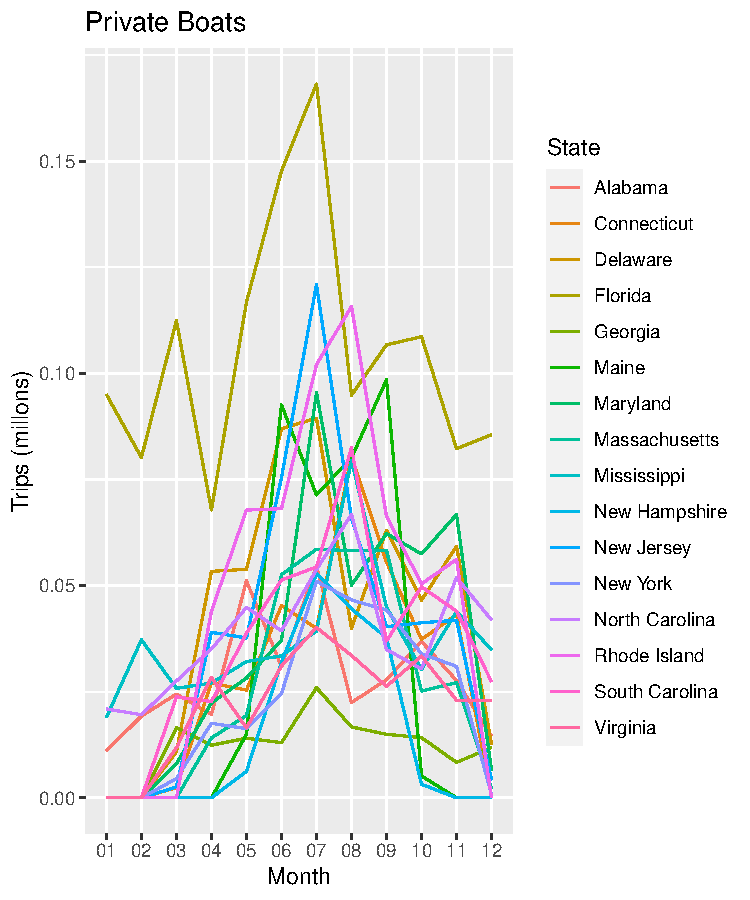
\includegraphics{C19PolicyRec_files/figure-latex/pTrips-1} 

}

\caption{2020 Monthly Marine Sportfishing Trips per Capita by State}\label{fig:pTrips-1}
\end{figure}
\begin{figure}

{\centering 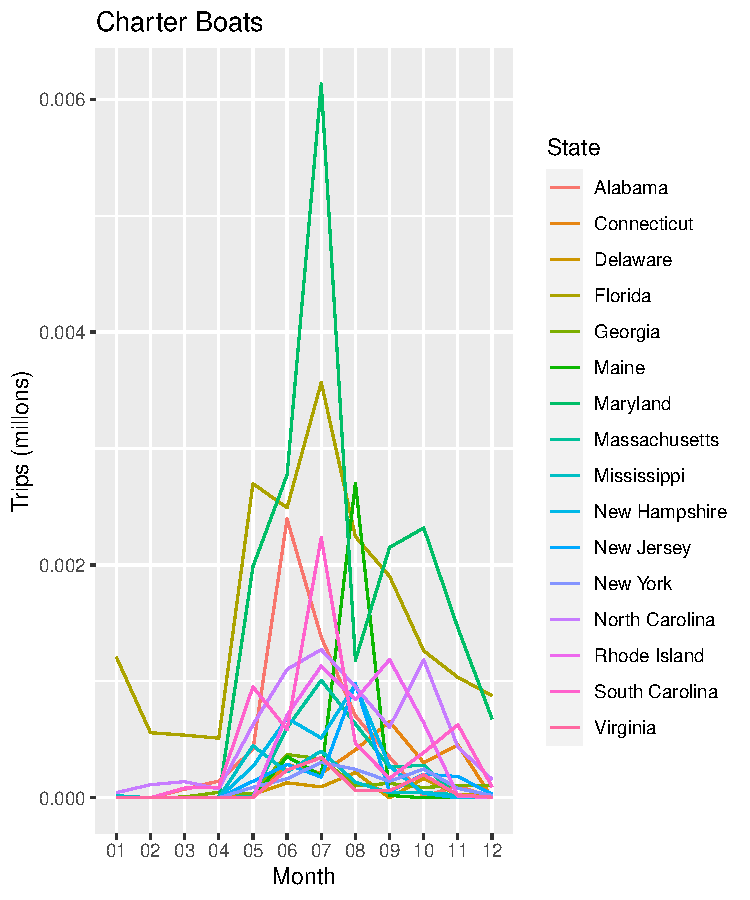
\includegraphics{C19PolicyRec_files/figure-latex/pTrips-2} 

}

\caption{2020 Monthly Marine Sportfishing Trips per Capita by State}\label{fig:pTrips-2}
\end{figure}
\begin{figure}

{\centering 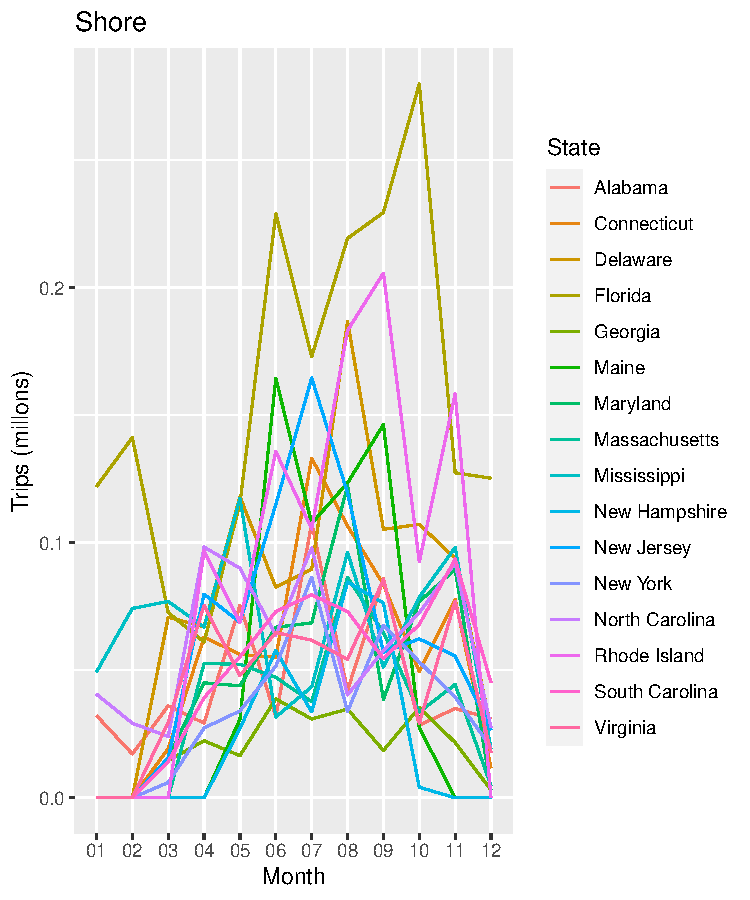
\includegraphics{C19PolicyRec_files/figure-latex/pTrips-3} 

}

\caption{2020 Monthly Marine Sportfishing Trips per Capita by State}\label{fig:pTrips-3}
\end{figure}

\begin{figure}

{\centering 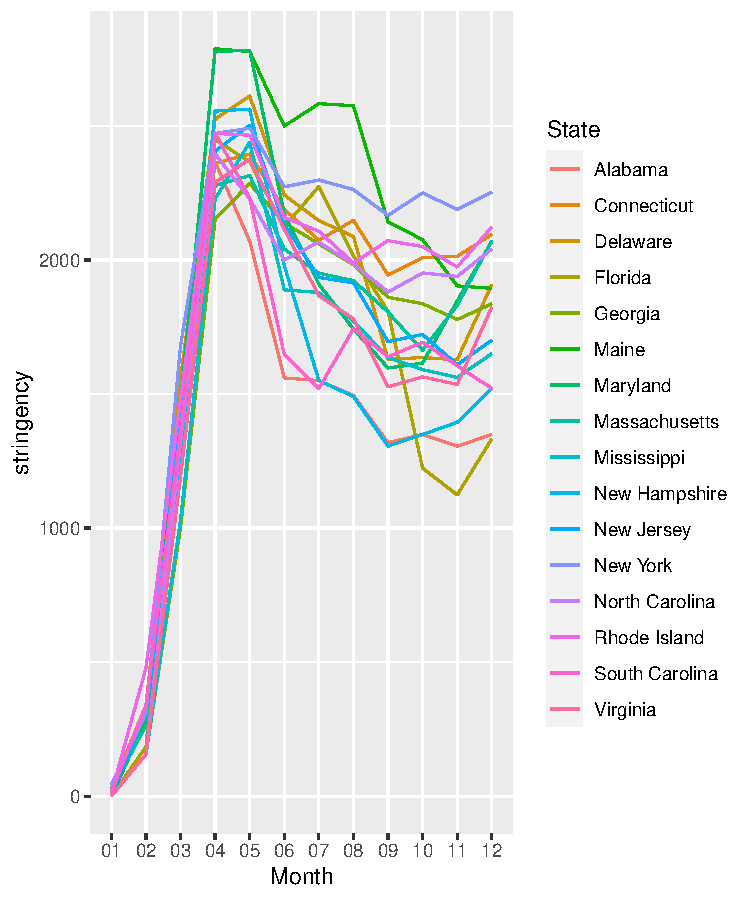
\includegraphics{C19PolicyRec_files/figure-latex/pString-1} 

}

\caption{Monthly 2020 stringency Index by State}\label{fig:pString}
\end{figure}

\begin{figure}

{\centering 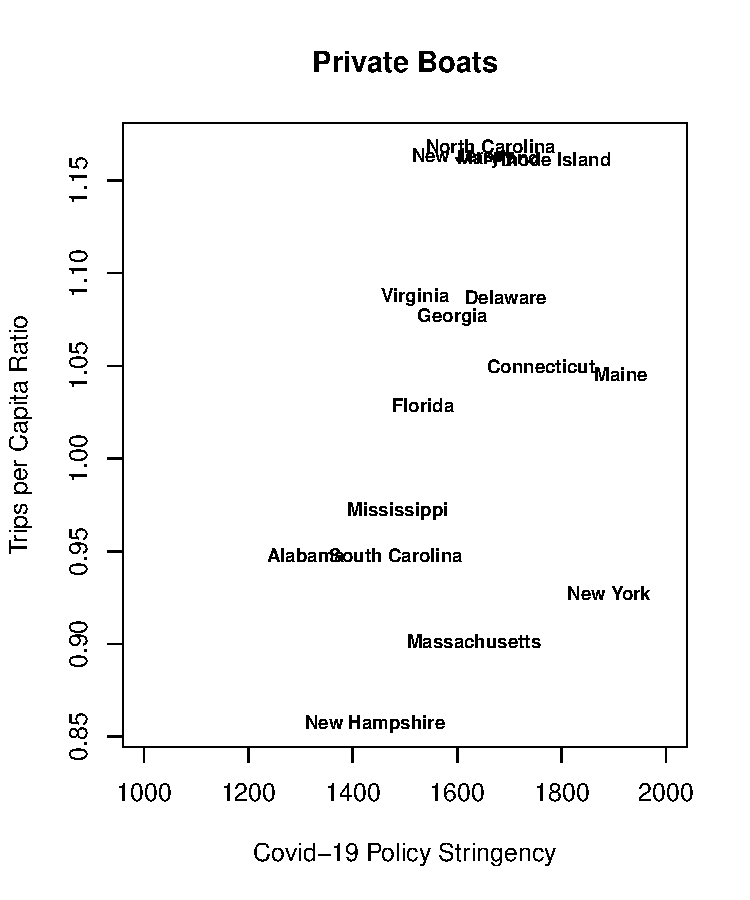
\includegraphics{C19PolicyRec_files/figure-latex/tripsVstring-1} 

}

\caption{Average Trips per Capita versus Covid-19 Policy Stringency}\label{fig:tripsVstring-1}
\end{figure}
\begin{figure}

{\centering 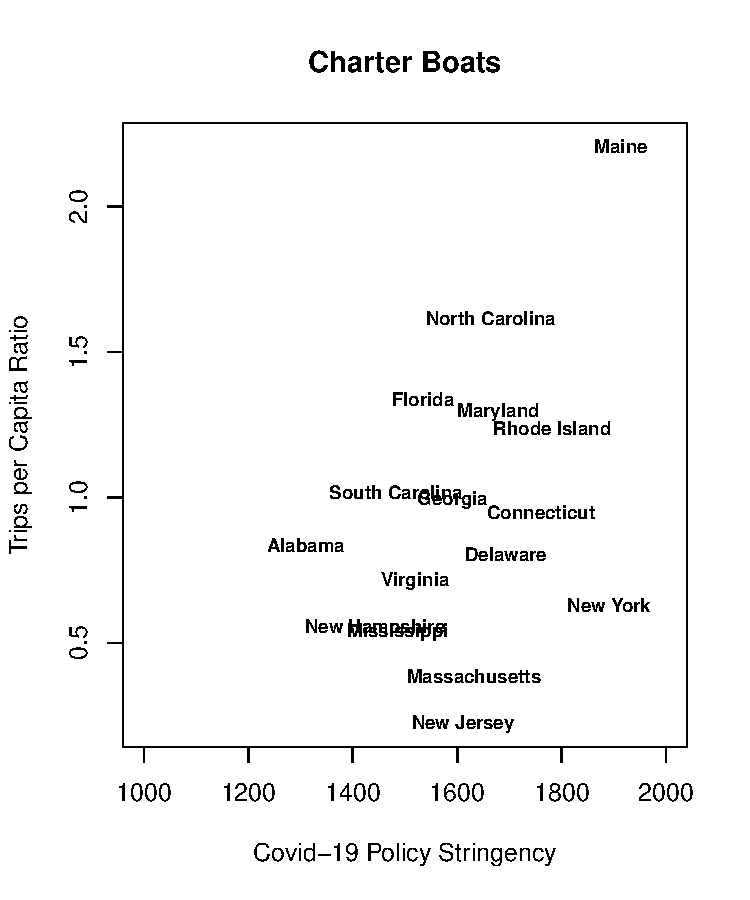
\includegraphics{C19PolicyRec_files/figure-latex/tripsVstring-2} 

}

\caption{Average Trips per Capita versus Covid-19 Policy Stringency}\label{fig:tripsVstring-2}
\end{figure}
\begin{figure}

{\centering 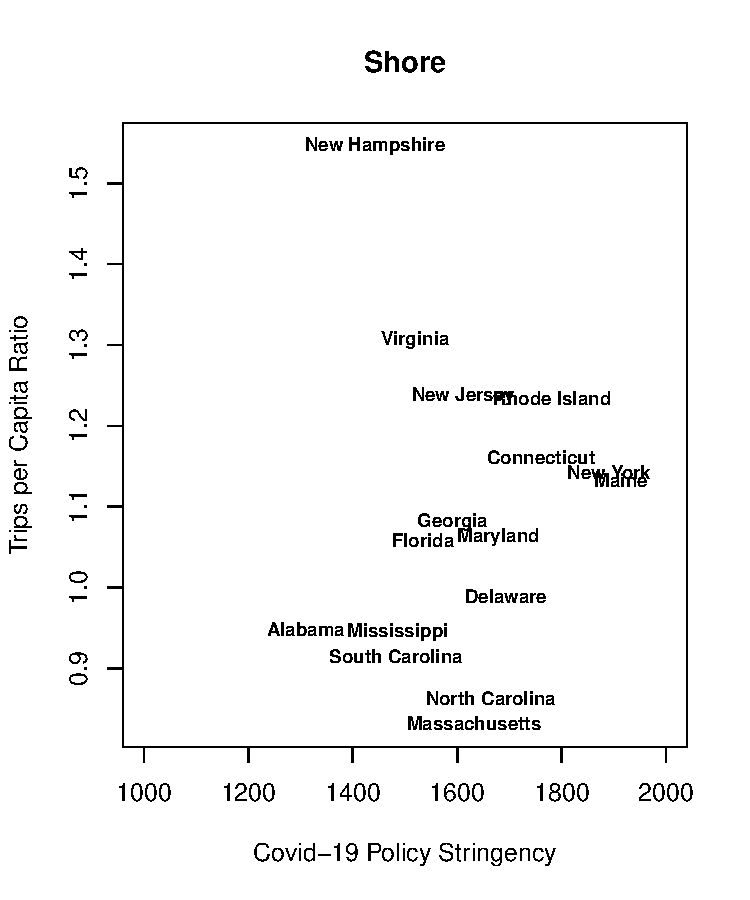
\includegraphics{C19PolicyRec_files/figure-latex/tripsVstring-3} 

}

\caption{Average Trips per Capita versus Covid-19 Policy Stringency}\label{fig:tripsVstring-3}
\end{figure}

\hypertarget{modeling-approach}{%
\subsection{Modeling Approach}\label{modeling-approach}}

Quasi-poisson regression estimated with mean equal to
\(exp(pop)*exp(xb)\) and variance equal to \(scale*mean\).

\hypertarget{results}{%
\section{Results}\label{results}}

Our results represent a composite effect of the actual local COVID
policies, as well as localized attitudes, risk tolerances, and beliefs
about COVID-19 which are correlated with COVID stringency. In
particular, we see the inverse-U relationship we find to be the outcome
of 2 countervailing pathways (laid out in the background section), (1)
stringency reduces available substitutes of indoor or high-density
outdoor activities, increasing the attractiveness of fishing, which is
the dominant force on the low-stringency side of the curve, and (2)
COVID risk makes even a relatively distanced activity, such as fishing,
less appealing compared to entirely in-home activities such as cooking,
backyard games, video games, etc., which is the dominating force on the
high-stringency side of the curve.

\begin{table}
\caption{Quasi-Poisson Fixed Effect Regression of Trips on Covid-19 Stringency by Mode}
\begin{center}
\begin{tabular}{l c c c}
\hline
 & Private & Charter & Shore \\
\hline
Intercept            & $-4.487 \; (0.137)^{***}$ & $-9.083 \; (0.227)^{***}$ & $-3.729 \; (0.130)^{***}$ \\
Connecticut          & $-0.006 \; (0.153)$       & $-0.947 \; (0.267)^{***}$ & $0.053 \; (0.151)$        \\
Delaware             & $0.335 \; (0.214)$        & $-2.021 \; (0.783)^{*}$   & $0.537 \; (0.198)^{**}$   \\
Florida              & $1.269 \; (0.102)^{***}$  & $0.893 \; (0.130)^{***}$  & $1.172 \; (0.102)^{***}$  \\
Georgia              & $-0.912 \; (0.146)^{***}$ & $-1.552 \; (0.223)^{***}$ & $-0.924 \; (0.146)^{***}$ \\
Maine                & $0.032 \; (0.214)$        & $-1.151 \; (0.449)^{*}$   & $0.006 \; (0.218)$        \\
Maryland             & $0.114 \; (0.130)$        & $0.907 \; (0.144)^{***}$  & $-0.024 \; (0.135)$       \\
Massachusetts        & $-0.022 \; (0.130)$       & $-0.028 \; (0.164)$       & $-0.145 \; (0.134)$       \\
Mississippi          & $0.265 \; (0.149)$        & $-1.052 \; (0.298)^{***}$ & $0.391 \; (0.144)^{**}$   \\
New Hampshire        & $-0.574 \; (0.269)^{*}$   & $-0.359 \; (0.309)$       & $-1.002 \; (0.327)^{**}$  \\
New Jersey           & $0.186 \; (0.119)$        & $0.163 \; (0.151)$        & $0.152 \; (0.120)$        \\
New York             & $-0.180 \; (0.114)$       & $-1.198 \; (0.170)^{***}$ & $-0.368 \; (0.117)^{**}$  \\
North Carolina       & $0.180 \; (0.117)$        & $-0.271 \; (0.159)$       & $0.381 \; (0.114)^{***}$  \\
Rhode Island         & $0.391 \; (0.202)$        & $-0.475 \; (0.363)$       & $0.478 \; (0.196)^{*}$    \\
South Carolina       & $0.243 \; (0.131)$        & $-0.126 \; (0.179)$       & $0.112 \; (0.135)$        \\
Virginia             & $-0.333 \; (0.133)^{*}$   & $-1.641 \; (0.248)^{***}$ & $-0.233 \; (0.130)$       \\
February             & $0.334 \; (0.125)^{**}$   & $0.191 \; (0.258)$        & $-0.012 \; (0.121)$       \\
March                & $0.366 \; (0.125)^{**}$   & $0.585 \; (0.238)^{*}$    & $0.070 \; (0.119)$        \\
April                & $0.909 \; (0.115)^{***}$  & $1.003 \; (0.226)^{***}$  & $0.721 \; (0.107)^{***}$  \\
May                  & $1.051 \; (0.113)^{***}$  & $1.902 \; (0.206)^{***}$  & $0.806 \; (0.105)^{***}$  \\
June                 & $1.358 \; (0.108)^{***}$  & $2.301 \; (0.201)^{***}$  & $1.073 \; (0.100)^{***}$  \\
July                 & $1.499 \; (0.107)^{***}$  & $2.344 \; (0.201)^{***}$  & $1.069 \; (0.100)^{***}$  \\
August               & $1.356 \; (0.108)^{***}$  & $2.075 \; (0.203)^{***}$  & $0.935 \; (0.102)^{***}$  \\
September            & $1.070 \; (0.111)^{***}$  & $1.464 \; (0.212)^{***}$  & $0.798 \; (0.104)^{***}$  \\
October              & $0.927 \; (0.114)^{***}$  & $1.289 \; (0.216)^{***}$  & $0.790 \; (0.104)^{***}$  \\
November             & $0.875 \; (0.115)^{***}$  & $1.203 \; (0.218)^{***}$  & $0.655 \; (0.106)^{***}$  \\
December             & $0.335 \; (0.126)^{**}$   & $0.659 \; (0.235)^{**}$   & $-0.045 \; (0.123)$       \\
Stringency/100       & $0.027 \; (0.013)^{*}$    & $0.026 \; (0.019)$        & $0.038 \; (0.013)^{**}$   \\
(Stringency/100)$^2$ & $-0.001 \; (0.001)^{*}$   & $-0.001 \; (0.001)$       & $-0.002 \; (0.001)^{**}$  \\
\hline
Scale                & $67644.479$               & $1926.588$                & $110073.475$              \\
Deviance             & $55884180.463$            & $1371580.349$             & $90756332.568$            \\
Num. obs.            & $768$                     & $768$                     & $768$                     \\
\hline
\multicolumn{4}{l}{\scriptsize{$^{***}p<0.001$; $^{**}p<0.01$; $^{*}p<0.05$. The base state is Alabama and the base Month is January.}}
\end{tabular}
\label{regResults}
\end{center}
\end{table}

\begin{figure}
\centering
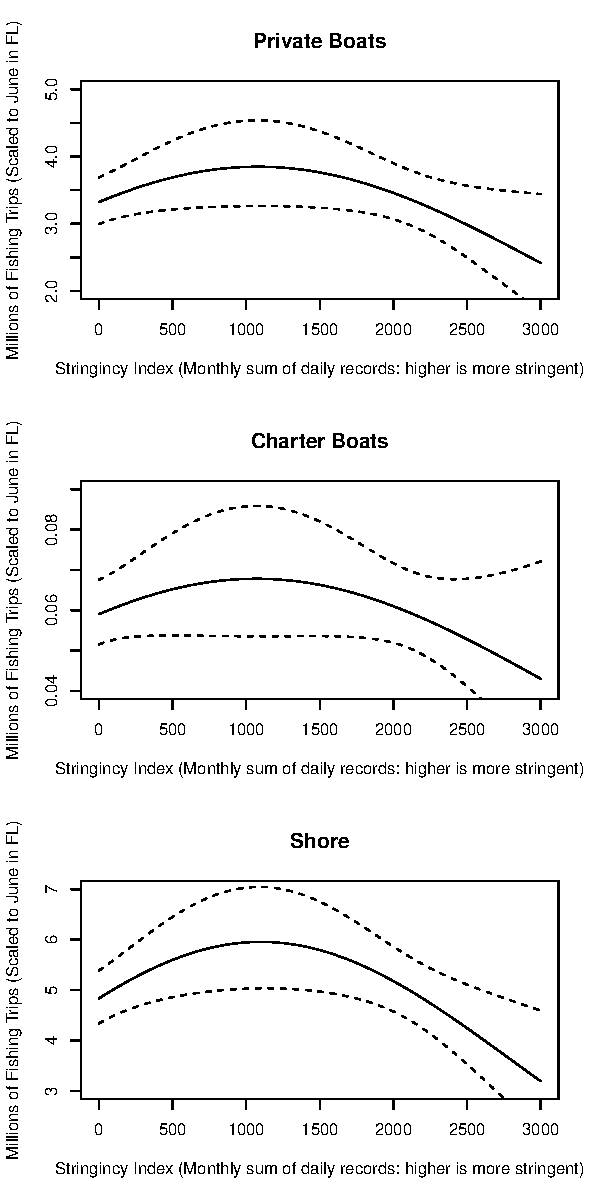
\includegraphics{C19PolicyRec_files/figure-latex/tripStringRel-1.pdf}
\caption{Predicted Trips as a Function of the Stringency Index}
\end{figure}

\hypertarget{references}{%
\section*{References}\label{references}}
\addcontentsline{toc}{section}{References}

{[}a{]}why not average? Different months have different numbers of days

\nolinenumbers


\end{document}
